\documentclass[fontsize=20pt]{scrartcl}
\usepackage[margin=0.5in, a4paper, landscape]{geometry}
\usepackage{tikz}
\usepackage{amsmath}
\usepackage{pgfplots}
\usepackage{siunitx}
\usetikzlibrary{calc,patterns,angles,quotes}
\begin{document}
The matrix $\begin{pmatrix}\sqrt{2}&-\sqrt{2}\\ \sqrt{2}&\sqrt{2}\end{pmatrix}$ performs a rotation of 45 degrees anti-clockwise about the origin. The matrix $\begin{pmatrix}1 &0\\0&-1\end{pmatrix}$ represents a reflection in the $x$-axis. The matrix $\begin{pmatrix}0&1\\-1&0\end{pmatrix}$ represents a rotation of 90 degrees clockwise about the origin. The matrix $\begin{pmatrix}-1&0\\0&1\end{pmatrix}$ performs a reflection in the $y$-axis. Work out the transformation matrices for the following transformations:
\newline
\newline
\begin{tabular}{p{13cm}p{13cm}}
Reflection in $y$-axis followed by rotation 45 degrees anti-clockwise
&.
\\\\\\\\\\\\
Rotation of 90 degrees clockwise followed by reflection in the $x$-axis
&.
\\\\\\\end{tabular}
\newpage
The matrix $\begin{pmatrix}\sqrt{2}&-\sqrt{2}\\ \sqrt{2}&\sqrt{2}\end{pmatrix}$ performs a rotation of 45 degrees anti-clockwise about the origin. The matrix $\begin{pmatrix}1 &0\\0&-1\end{pmatrix}$ represents a reflection in the $x$-axis. The matrix $\begin{pmatrix}0&1\\-1&0\end{pmatrix}$ represents a rotation of 90 degrees clockwise about the origin. The matrix $\begin{pmatrix}-1&0\\0&1\end{pmatrix}$ performs a reflection in the $y$-axis. Work out the transformation matrices for the following transformations:
\newline
\newline
\begin{tabular}{p{13cm}p{13cm}}
Rotation of 45 degrees anti-clockwise, then reflection in $x$-axis, then rotation of 90 degrees clockwise
&.
\\\\\\\\\\\\
Rotation of 90 degrees clockwise followed by reflection in the $y$-axis followed by reflection in the $x$-axis
&.
\\\\\\\end{tabular}
\newpage
Work out the single transformation equivalent to reflection in $y$-axis followed by rotation 45 degrees anti-clockwise
\newline
\newline
\begin{tabular}{p{13cm}p{13cm}}
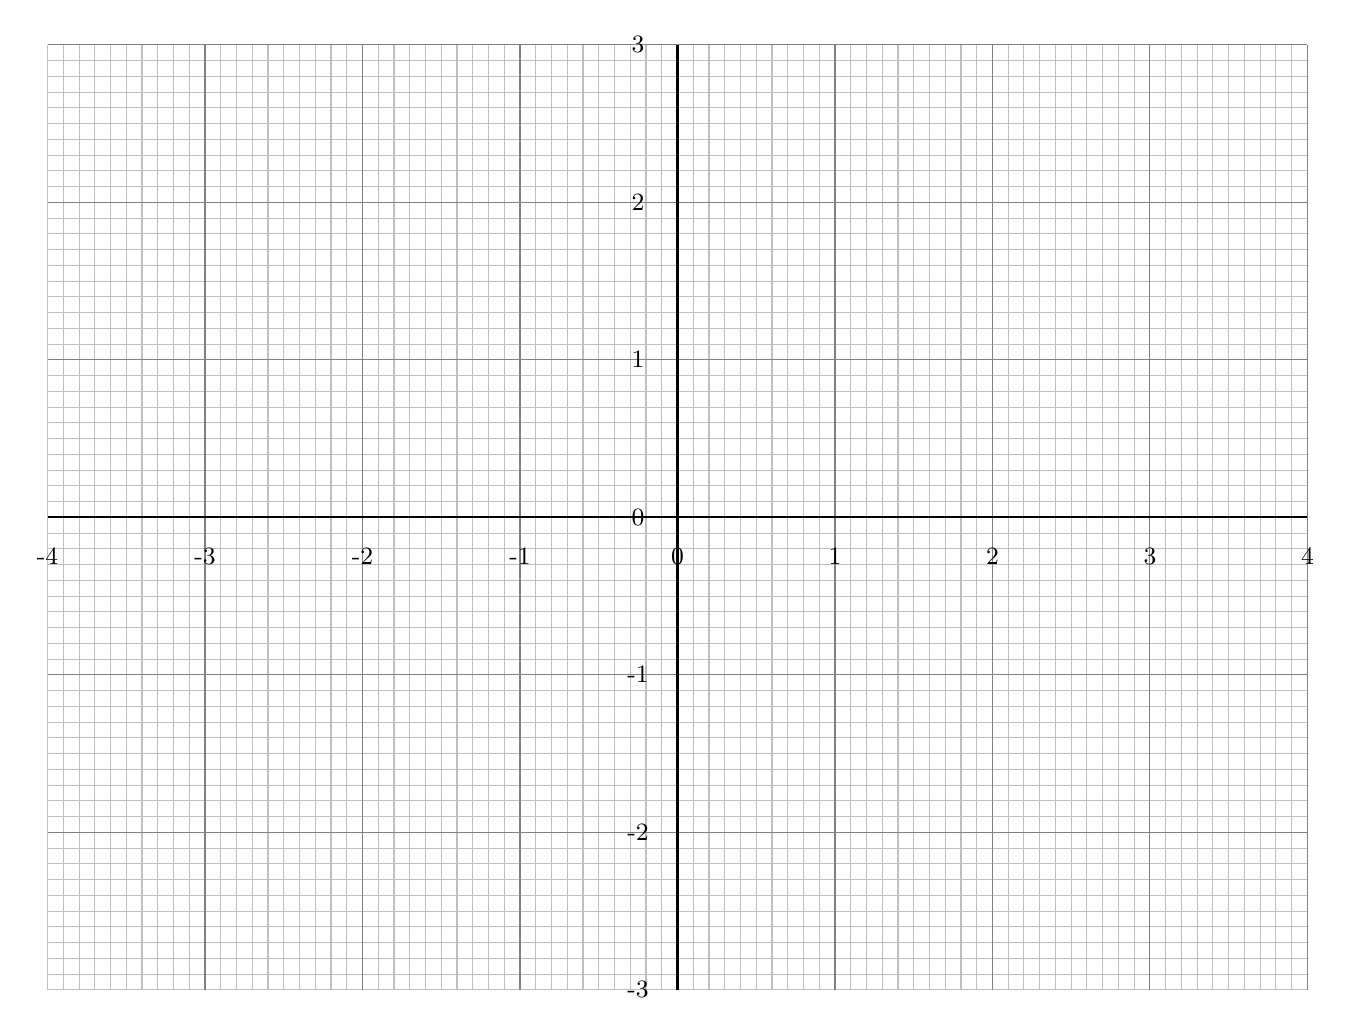
\begin{tikzpicture}
\draw[thin, step=0.2cm,color=lightgray] (-8,-6) grid (8,6);
\draw[thin, step=2cm,color=gray] (-8,-6) grid (8,6);
\draw[thick] (-8,0)--(8,0);
\draw[thick] (0,6)--(0,-6);
\foreach \x in {-4,...,4}{
  \node at (\x*2,-0.5)  {\small{\x}};
}
\foreach \y in {-3,...,3}{
  \node at (-0.5,\y*2)  {\small{\y}};
}
\end{tikzpicture}
&\\\\\\
\end{tabular}
\newpage
Work out the single transformation equivalent to rotation 180 degrees about the origin followed by reflection in $x$-axis 
\newline
\newline
\begin{tabular}{p{13cm}p{13cm}}
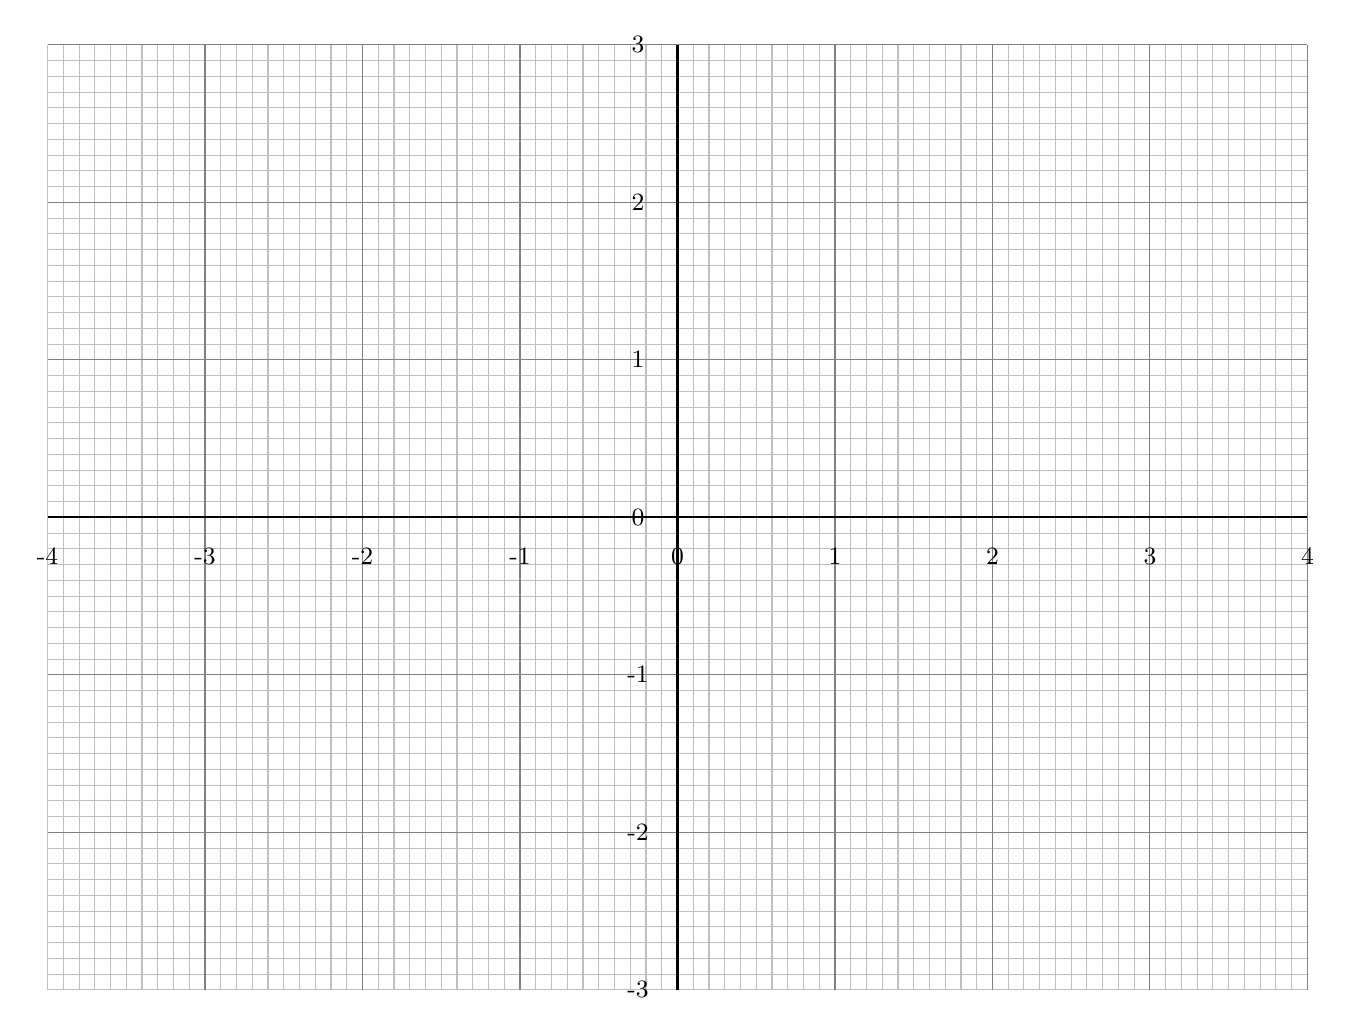
\begin{tikzpicture}
\draw[thin, step=0.2cm,color=lightgray] (-8,-6) grid (8,6);
\draw[thin, step=2cm,color=gray] (-8,-6) grid (8,6);
\draw[thick] (-8,0)--(8,0);
\draw[thick] (0,6)--(0,-6);
\foreach \x in {-4,...,4}{
  \node at (\x*2,-0.5)  {\small{\x}};
}
\foreach \y in {-3,...,3}{
  \node at (-0.5,\y*2)  {\small{\y}};
}
\end{tikzpicture}
&
\end{tabular}
\end{document}
